\documentclass[a4paper,11pt]{article}
\usepackage[T1]{fontenc}
\usepackage[utf8]{inputenc}
\usepackage{graphicx}
\usepackage{xcolor}


\usepackage{amsmath,amssymb,amsthm,textcomp}
\usepackage{enumerate}
\usepackage{multicol}
\usepackage{tikz}
\usepackage[english, russian]{babel}

\usepackage{geometry}
\geometry{total={210mm,297mm},
	left=25mm,right=25mm,%
	bindingoffset=0mm, top=20mm,bottom=20mm}


% custom footers and headers
\usepackage{fancyhdr}
\pagestyle{fancy}
\lhead{\footnotesize Линейная алгебра и геометрия}
\chead{}
\rhead{\scriptsize ФКН НИУ ВШЭ, 2016/2017 учебный год, 1 курс ПМИ, Егерев Артем}
\lfoot{}
\cfoot{}
\renewcommand{\headrulewidth}{0pt}
\renewcommand{\footrulewidth}{0pt}

%%%----------%%%----------%%%----------%%%----------%%%


\begin{document}
\textbf{\large Задача 1}
\medskip\hrule\medskip
\textit{Для квадратичной формы}
\begin{gather*}
Q(x_1, x_2, x_3) = x_1^2(13b - 18) + x_2^2(-5 + b) + x_3^2(5b - 5) + 2x_1x_2(-3b + 6) + 2x_1x_3(-b - 6) + 2x_2x_3(-1 - b)
\end{gather*}
\textit{выясните при каких значениях параметра $ b $ она является положительно определенной, а при каких $ - $ отрицательно определенной?} \\ \\
Составим матрицу квадратичной формы, и посчитаем ее угловые миноры:
\begin{gather*}
M = 
\begin{pmatrix}
13b - 18 & -3b + 6 & -b - 6 \\[2pt]
-3b + 6 & -5 + b & -1 - b\\[2pt]
-b - 6 & -1 - b & 5b - 5
\end{pmatrix}
\end{gather*}
\begin{itemize}
\item $ \Delta_1 = 13b - 18 = 13(b - \frac{18}{13})$ \\[2pt]
\item $ \Delta_2 = (13b - 18)(-5 + b) - (-3b + 6)^2 = 4 b^2 - 47 b + 54 = 4(b - \frac{47}8 + \frac{\sqrt{1345}}8)(b - \frac{47}8 - \frac{\sqrt{1345}}8)$ \\[2pt]
\item $ \Delta_3 = (13b - 18)((-5 + b)(5b - 5) - (-1 - b)^2) - (-3b + 6)((-3b + 6)(5b - 5) - (-1 - b)(-b - 6)) \; + \\[2pt] 
 + \;(-b - 6)((-3b + 6)(-1 - b) - (-5 + b)(-b - 6)) = -300 b (b - 2) $
\end{itemize}
Исходя из критерия Сильвестра, для того чтобы квадратичная форма была положительно определена требуется:
\begin{itemize}
\item $ \Delta_1 > 0 \Rightarrow b > \frac{18}{13}$
\item $ \Delta_2 > 0 \Rightarrow b \in (-\infty, \frac{47}8 - \frac{\sqrt{1345}}8) \cup (\frac{47}8 + \frac{\sqrt{1345}}8, \infty)$
\item $ \Delta_3 > 0 \Rightarrow b \in (0, 2)$
\end{itemize}
$ \Rightarrow b \in \varnothing $ \\ Аналагично, для того чтобы матрица была отрицательно определена, согласно критерию Сильвестра, получаем:
\begin{itemize}
\item $ \Delta_1 < 0 \Rightarrow b < \frac{18}{13}$
\item $ \Delta_2 > 0 \Rightarrow b \in (-\infty, \frac{47}8 - \frac{\sqrt{1345}}8) \cup (\frac{47}8 + \frac{\sqrt{1345}}8, \infty)$
\item $ \Delta_3 < 0 \Rightarrow b \in (-\infty, 0) \cup (2, \infty)$
\end{itemize}
$ \Rightarrow b \in (-\infty, 0) $
\newpage





%%%----------%%%----------%%%----------%%%----------%%%




\textbf{\large Задача 2}
\medskip\hrule\medskip
\textit{Подпространство $ U $ евклидова пространства $ \mathbb{R}^4 $ задано уравнением $ x_1 - 5x_2 - 3x_3 - \\ - x_4 = 0 $}
\begin{itemize}
\item \textit{Постройте в $ U $ ортонормированный базис}
\item \textit{Для вектора $ v = (1, 2, 0, 0) $ найдите его проекцию на $ U $, его ортоганальную составляющую относительно $ U $ и расстояние от него до $ U $.}
\end{itemize} 
Для начала найдем простой базис (не обязательно ортонормированный) в подпространстве $ U $. Для этого найдем ФСР для СЛУ:
\begin{gather*}
\begin{cases}
x_1 - 5x_2 - 3x_3 - x_4 = 0
\end{cases}
\end{gather*}
Взяв за свободные переменные последние 3, получаем вектора: $p =  (1, 0, 0, 1), (3, 0, 1, 0), (5, 1, 0, 0) $. Отлично, теперь данный базис следует ортонормировать.
\begin{itemize}
\item $ u_1 = \frac{p_1}{|p_1|} = (\frac1{\sqrt{2}}, 0, 0, \frac1{\sqrt{2}}) $
\item $ u_2' = p_2 - (u_1, p_2)u_1 = (3, 0, 1, 0) - \frac{3}{\sqrt{2}}(\frac1{\sqrt{2}}, 0, 0, \frac1{\sqrt{2}}) = (\frac32, 0, 1, -\frac32)  \\[2pt]
u_2 = \frac{u_2'}{|u_2'|} = (\frac3{\sqrt{22}}, 0, \frac2{\sqrt{22}}, -\frac3{\sqrt{22}})$
\item $ u_3' = p_3 - (u_1, p_3)u_1 = (5, 1, 0, 0) - \frac5{\sqrt{2}}(\frac1{\sqrt{2}}, 0, 0, \frac1{\sqrt{2}}) = (\frac52, 1, 0, -\frac52) \\[2pt]
u_3'' = u_3' - (u_2, u_3')u_2 = (\frac52, 1, 0, -\frac52) - \frac{15}{\sqrt{22}}(\frac3{\sqrt{22}}, 0, \frac2{\sqrt{22}}, -\frac3{\sqrt{22}}) =  (\frac5{11}, 1, -\frac{15}{11}, -\frac{5}{11})\\[2pt]
u_3 = \frac{u_3''}{|u_3''|} = (\frac5{6\sqrt{11}}, \frac{11}{6\sqrt{11}}, -\frac{5}{2\sqrt{11}}, -\frac5{6\sqrt{11}})$ 
\end{itemize}
Для решения следующего пункта вспомним, что вектор $ v = (1, 2, 0, 0) = m + u $, где вектор $ m $ принадлежит дополнению $ U $ до $ \mathbb{R}^4 $, $ u \in U $. \\[2pt]
Отметим, что вектор $ (1, -5, -3, -1) $ перпендикулярен $ U $, а значит и образует базис в $ M $ (это следует из уравнения задания подпространства).
\begin{gather*}
v = x_1 \times p_1 + x_2 \times p_2 + x_3 \times p_3 + x_4 \times m \\
\begin{pmatrix}
1 & 3 & 5 & 1 & \vrule & 1 \\[2pt]
0 & 0 & 1 & -5 & \vrule &  2 \\[2pt]
0 & 1 & 0 & -3 & \vrule & 0 \\[2pt]
1 & 0 & 0 & -1 & \vrule & 0
\end{pmatrix}
\longrightarrow 
\begin{pmatrix}
1 & 0 & 0 & -1 & \vrule & 0 \\[2pt]
0 & 0 & 1 & -5 & \vrule &  2 \\[2pt]
0 & 1 & 0 & -3 & \vrule & 0 \\[2pt]
1 & 3 & 5 & 1 & \vrule & 1 
\end{pmatrix}
\longrightarrow
\begin{pmatrix}
1 & 0 & 0 & -1 & \vrule & 0 \\[2pt]
0 & 0 & 1 & -5 & \vrule &  2 \\[2pt]
0 & 1 & 0 & -3 & \vrule & 0 \\[2pt]
0 & 3 & 5 & 2 & \vrule & 1 
\end{pmatrix}
\\
\begin{pmatrix}
1 & 0 & 0 & -1 & \vrule & 0 \\[2pt]
0 & 0 & 1 & -5 & \vrule &  2 \\[2pt]
0 & 1 & 0 & -3 & \vrule & 0 \\[2pt]
0 & 0 & 5 & 11 & \vrule & 1 
\end{pmatrix}
\longrightarrow
\begin{pmatrix}
1 & 0 & 0 & -1 & \vrule & 0 \\[2pt]
0 & 0 & 1 & -5 & \vrule &  2 \\[2pt]
0 & 1 & 0 & -3 & \vrule & 0 \\[2pt]
0 & 0 & 0 & 36 & \vrule & 9 
\end{pmatrix}
\end{gather*}
Отсюда следуют, что $ x_4 = \frac14, x_3 = 2 + 5x_4 = \frac{13}{4}, x_2 = 3x_4 = \frac34, x_1 = x_4 = \frac14 $. Тогда проекция на $ U $ это просто: $  x_1 \times p_1 + x_2 \times p_2 + x_3 \times p_3  = \frac14(1, 0, 0, 1) + \frac34(3, 0, 1, 0) + \frac{13}4(5, 1, 0, 0) = (\frac{75}4, \frac{13}4, \frac34, \frac14)$ \\[2pt]
Ортогональная проекция есть просто $ x_4 \times m  = \frac14(1, -5, -3, -1) = (\frac14, -\frac54, -\frac34, -\frac14)$ \\
Отметим, что минимальное расстояние есть просто длина ортогональной проекции, простыми вычислениями получаем:
\begin{gather*}
\rho = \big\arrowvert(\frac14, -\frac54, -\frac34, -\frac14)\big\arrowvert = \frac14\sqrt{1^2 + 5^2 + 3^2 + 1^2} = \frac32
\end{gather*}
\newpage





%%%----------%%%----------%%%----------%%%----------%%%




\textbf{\large Задача 3}
\medskip\hrule\medskip
\textit{Составьте уравнение прямой в $ \mathbb{R}^3 $, параллельной плоскости $ x + 4y - 3z = 0 $, проходящей через точку $ (1, 2, -2) $ и пересекающей прямую $ x = -3t + 4, y = 3t - 3, z = 2t - 2 $.} \\ \\
Наша будующая прямая представима в виде:
\begin{gather*}
\begin{pmatrix}
x \\
y \\
z 
\end{pmatrix}
 = 
\begin{pmatrix}
1 \\
2 \\
-2 
\end{pmatrix}
+ 
\begin{pmatrix}
a \\
b \\
c 
\end{pmatrix}
t_1
\end{gather*}
так как прямая однозначно задается точкой, через которую она проходит, и координатами направляющего вектора. Для начала, попробуем использовать условие того, что наша прямая параллельна плоскости $ x + 4y - 3z = 0 $. Это значит, что вектор нормали к этой плоскости перпендикулярен направляющему вектору нашей прямой, то есть скалярное произведение равно 0:
\begin{gather*}
a + 4b - 3c = 0
\end{gather*}
Так же необходимо задать формулу вспомогательной прямой, и записать условие того, что наши две прямые пересекаются в какой-то точке. 
\begin{gather*}
\begin{pmatrix}
x \\
y \\
z 
\end{pmatrix}
= 
\begin{pmatrix}
4 \\
-3 \\
-2 
\end{pmatrix}
+ 
\begin{pmatrix}
-3 \\
3 \\
2 
\end{pmatrix}
t_2 \\
\begin{pmatrix}
1 \\
2 \\
-2 
\end{pmatrix}
+ 
\begin{pmatrix}
a \\
b \\
c 
\end{pmatrix}
t_1
= 
\begin{pmatrix}
4 \\
-3 \\
-2 
\end{pmatrix}
+ 
\begin{pmatrix}
-3 \\
3 \\
2 
\end{pmatrix}
t_2 \Rightarrow 
\begin{pmatrix}
at_1 \\
bt_1 \\
bt_1 
\end{pmatrix}
= \begin{pmatrix}
3 \\
-5 \\
0 
\end{pmatrix}
+ 
\begin{pmatrix}
-3 \\
3 \\
2 
\end{pmatrix}
t_2 \\
(a + 4b - 3c)t_1 = 0
\end{gather*}
\begin{itemize}
\item $ at_1 = 3 - 3t_2 $
\item $ bt_1 = -5 + 3t_2 $
\item $ ct_1 = 2t_2 $
\end{itemize}
\begin{gather*}
(a + 4b - 3c)t_1 = (3 - 3t_2) + 4(-5 + 3t_2) - 6t_2 = 3t_2 - 17 = 0 \Rightarrow t_2 = \frac{17}3 \Rightarrow
\end{gather*}
\begin{itemize}
\item $ A = at_1 = -14 $
\item $ B = bt_1 = 12 $
\item $ C = ct_1 = \frac{34}3 $
\end{itemize}

Отметим так же, что нам важны координаты направляющего вектора с точностью до пропорциональносит, поэтому можем уже выписывать наш ответ:
\begin{gather*}
\begin{pmatrix}
x \\
y \\
z 
\end{pmatrix}
= 
\begin{pmatrix}
1 \\
2 \\
-2 
\end{pmatrix}
+ 
\begin{pmatrix}
-14 \\
12 \\
\frac{34}3
\end{pmatrix}
t
\end{gather*}
\newpage








%%%----------%%%----------%%%----------%%%----------%%%




\textbf{\large Задача 4}
\medskip\hrule\medskip
\textit{Дан куб $ ABCDA'B'C'D' $ со стороной 6. Точка $ F \; - $ середина ребра $ BB' $, а точка $ E $ лежит на ребре $ BB' $, причем $ BE : EB' = 4  :  7 $. Найдите угол и расстояние между прямыми $ AE $ и $ D'F $. } 
\begin{center}
	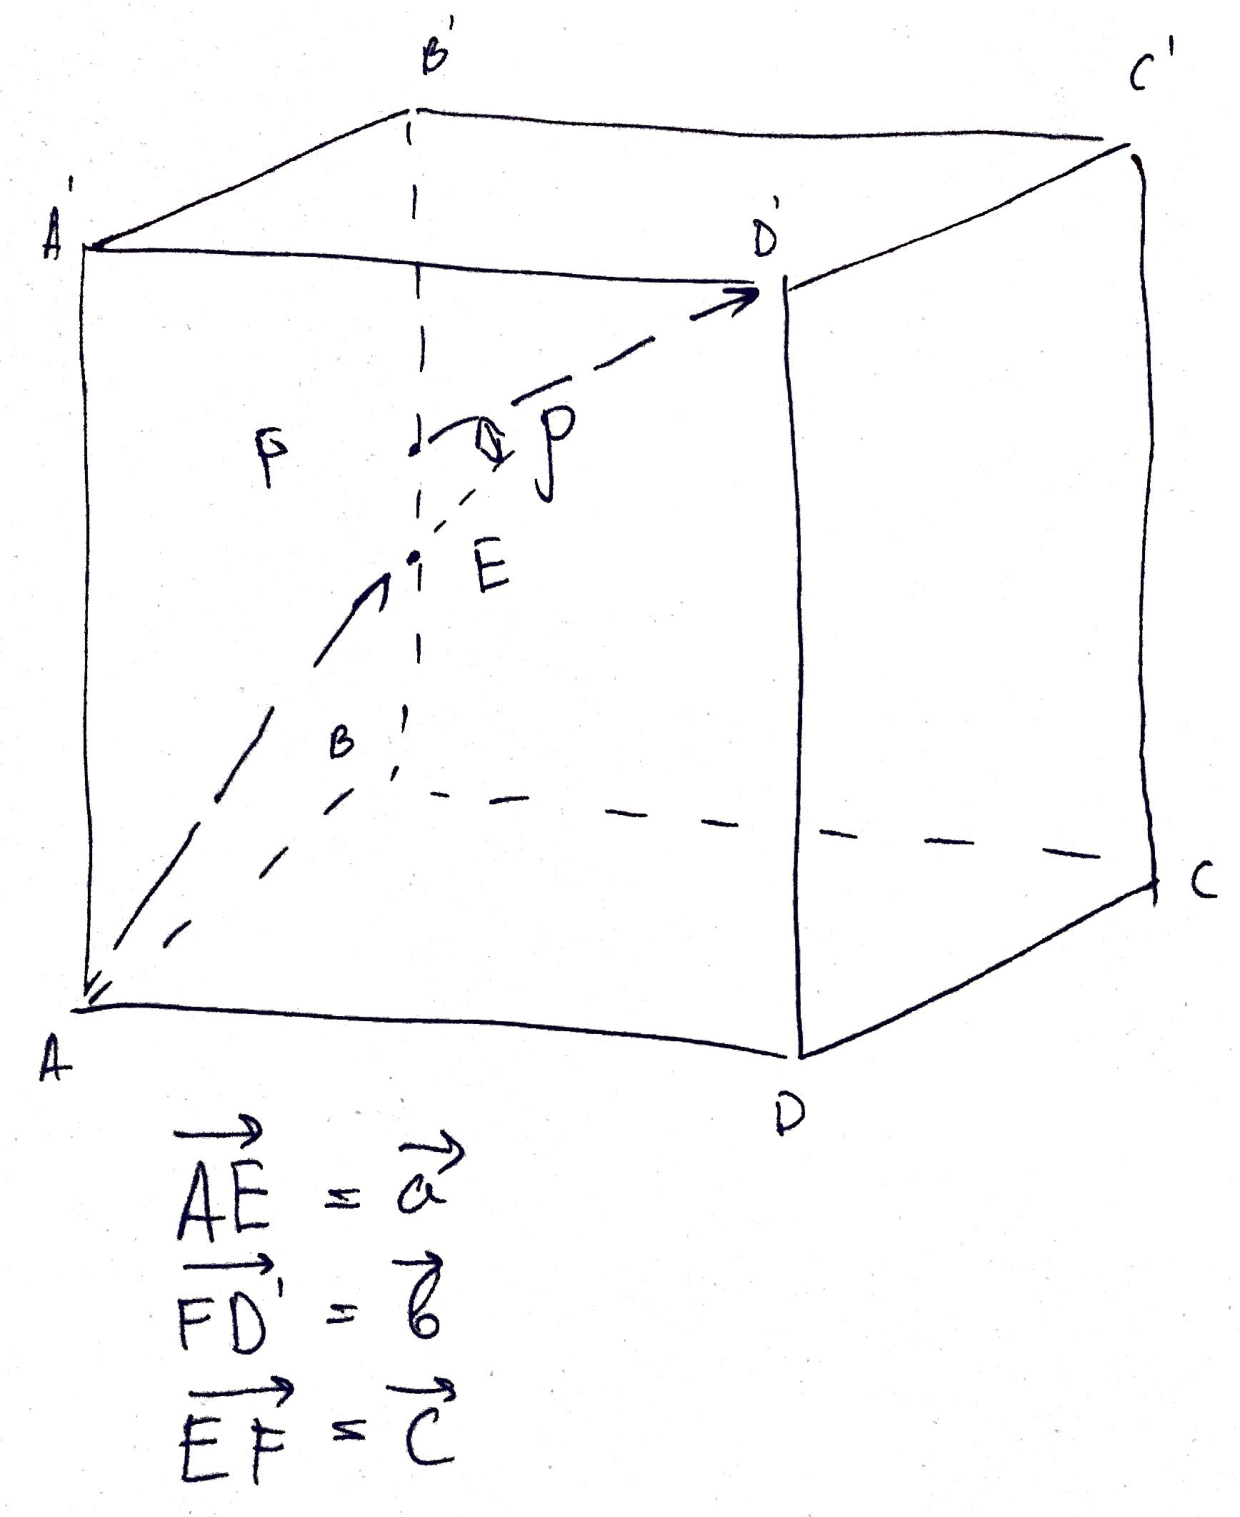
\includegraphics[height = 90mm]{cub.pdf	}
\end{center}
Введем координаты, с началом в точке $ A $.
\begin{gather*}
A (0, 0, 0) \quad E (0, 6, \dfrac{24}{11}) \quad F (0, 6, 3) \quad D' (6, 0, 6)
\end{gather*}   
Направляющими прямых будут являться вектора $ AE = a = (0, 6, \dfrac{24}{11}) \; FD' = b = (6, -6, 3)$ \\
Тогда угол между скрещивающимеся кривыми есть просто угол между их направляющими векторами:
\begin{gather*}
cos \alpha = abs(\frac{(a, b)}{|a||b|}) = \frac{\frac{324}{11}}{\frac{6\sqrt{137}}{11} \cdot 9} = \frac{6}{\sqrt{137}}
\end{gather*}
Обозначим вектор, равный расстоянию между прямыми за $ \rho $. Тогда $ \rho $ расскладывается на три вектора: вдоль первой прямой, вдоль второй и вектор по прямой, непосредственно соединяющей наши прямые : $ EF (0, 0, \frac9{11}) $.
\begin{gather*}
\rho = \alpha a + \beta b + EF
\end{gather*}
Так как $ \rho $ это вектор-расстояние, то он перпендикулярен каждому направляющему вектору.
\begin{gather*}
(\rho, a) = 0 \qquad (\rho, b) = 0
\end{gather*}
Составим сисетму:
\begin{gather*}
\begin{cases}
\alpha \frac{4932}{121} - \beta\frac{324}{11} + \frac{216}{121}= 0 \\[2pt]
-\alpha \frac{324}{11} + 81\beta + \frac{27}{11} = 0
\end{cases} \Rightarrow
\begin{cases}
\alpha = -\frac{9}{101} \\ \beta = -\frac{19}{303}
\end{cases} \\
\rho =  -\frac{9}{101} (0, 6, \dfrac{24}{11}) - \frac{19}{303}(6, -6, 3) + (0, 0, \frac{9}{11}) = (-\frac{38}{101}, -\frac{16}{101}, \frac{44}{101})
\end{gather*}
Расстояние есть длина этого вектора, то есть $ |\rho| = \frac{6}{\sqrt{101}} \approx 0.597022 $




\end{document}